\chapter{Rozbor řešené problematiky}

\section{Webové portály}
Webový portál je druh webové stránky, která shromažďuje informace z vícero různých zdrojů a uživateli ty nejrelevantnější informace prezentuje uživateli shromážděné na jednom místě~\cite{bib:portal-liferay}.

Zpravidla je umožněno na portálu v těchto informací vyhledávat. Velmi časté je také zakomponování autentizace uživatele a podle jeho role jsou mu zpřístupněny různé části daného portálu~\cite{bib:portal-indiana}. 

\blindtext[2]

\subsection{CORDIS}
\emph{Tato kapitola čerpá z~\cite{bib:cordis}}.
CORDIS (\emph{The Community Research and Development Information Service}) je portál provozovaný Evropskou Unií (dále jen EU) sloužící jako hlavní zdroj výsledků projektů, sponzorovaných v rámci programů EU pro výzkum a inovaci. Na jednom místě veřejně poskytuje informace jak o těchto projektech, tak i o jejích účastnících, o hlášeních, vědeckých zprávách a publikacích.
\blindtext

\subsection{Funding and Tenders}
\blindtext



\section{Vývoj webu}
\emph{Tato kapitola čerpá z~\cite{bib:web-development}}.

Tvorba webových stránek se obecně rozlišuje do dvou celků zvaných \emph{frontend} a \emph{backend}.

Frontendová část webu je to, co uživatel vidí, když stránku navštíví. Sestavení této části se v žádném případě neobejde bez značkovacího jazyka HTML (\emph{Hypertext Markup Language}), který udává strukturu a obsah webové stránky. Další nedílnou součástí jsou kaskádové styly neboli CSS (\emph{Cascading Style Sheets}). Ty se starají o to, jak bude obsah stránky esteticky působit. Další součástí, se kterou se setkáte téměř na každém webu je skriptovací jazyk JavaScript, který umožňuje webové stránky obohatit o interaktivitu.
Zpracování této části webu probíhá v klientovi - tedy internetovému prohlížeči uživatele. Na základě toto faktu se lze každé stránce na internetu \uv{nahlédnout pod pokličku} a zdrojové kódy frontendové části zobrazit, ve většině případů i rovnou v internetovém prohlížeči upravit, což má samozřejmě vliv jen pro současného uživatele a ostatním návštěvníkům se tyto změnu neprojeví.

Oproti tomu backendová část je od uživatele izolována a zdrojové kódy pro něj nejsou přístupné, pokud je sám autor někde nezveřejní. Jejich interpretace totiž probíhá přímo na serveru a ten poté klientovi odešle již zpracovanou frontendovou část. Výběr technologie implementace backendové části je podstatně rozmanitější, patří mezi ně například Python, PHP, Java, C#, C++, .NET, Ruby a další. Díky prostředí Node.js\footnote{Node.js: \url{https://nodejs.org/en/}} lze ale využít i dříve zmiňovaný JavaScript, který sám o sobě pro tento účel není primárně určen. 

\subsection{MVC architektura}
%[https://pdfs.semanticscholar.org/9077/6c1fd8c2c4dbd13b85f22e7c8c8f83331758.pdf 27.4.]
Většinu aplikací lze obecně rozdělit na tři hlavní celky - data, rozhraní a logiku. V anglickém jazyce se tyto celky dají nazvat pomocí slov \emph{model}, \emph{view} a \emph{controller} (zkratka MVC). Historie této architektury sahá až do sedmdesátých let, nicméně je v dnešním světe stále naprostým standardem vývoje.

\begin{figure}[H]
	\centering
	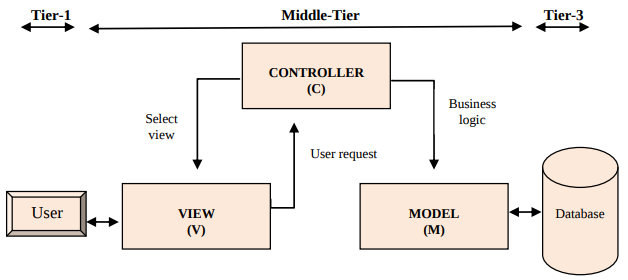
\includegraphics[width=\textwidth]{images/mvc.png}
	\caption{Diagram toku akcí při využití MVC architektury}
	\label{mvc}
\end{figure}

\begin{itemize}
\item Pojmem pohled (\emph{view}) se označuje uživatelské rozhraní (například stránka zobrazená v prohlížeči), tato vrstva prezentuje data a je to také jediná vrstva, s kterou uživatel přímo komunikuje. Akce provedené v pohledu se předají kontroleru ke zpracovaní.
\item Kontroler (\emph{controller}) se chová jako prostředník mezi daty a rozhraním, zpracovává požadavky uživatele a provede s modelem potřebné akce. Ve většině případu po provedené akci kontroler znovu obnoví pohled.
\item Model je obvykle objekt obsahující patřičná data z databáze. Zprostředkovává jak jejich získání, tak i ukládání. Mimo to může být objekt obohacen i o funkce, zpracovávající tyto data (například může převádět Unixový čas do formátu lépe čitelného pro člověka). 
\end{itemize}


Oddělením těchto celků je zajištěna lepší organizovanost zdrojových kódů a tím je usnadněn rychlejší vývoj. Jednotlivé celky jsou také lehčeji znovupoužitelné a práce programátorů na nich může probíhat souběžně. Rozdělením je také možné pro jeden pohled mít pohledů hned několik. Další pohledy mohou přibývat nebo naopak ty stávající mohou být smazány a na databázi aplikace to nebude mít žádný vliv.

\subsection{Responzivita}
\blindtext[2]

\section{Boostrap}
%[https://books.google.cz/books?hl=cs&lr=&id=iktVCgAAQBAJ&oi=fnd&pg=PP1&dq=bootstrap+css&ots=ZsIQ6TuKo-&sig=8AdB4nVzidu9ou2fX0LWq4TAn_U&redir_esc=y#v=onepage&q=bootstrap%20css&f=true 1.5.]
Bootstrap\footnote{Bootstrap: \url{https://getbootstrap.com/}} je frontendový framework pro snadný vývoj webových stránek. Je vyvíjen společností Twitter, která jej v roce 2010 vydala jako otevřený software. Jen dva roky poté se Bootstrap stal nejoblíbenějším projektem na stránce GitHub. Bootstrap se skládá převážně z kaskádových stylů, ale interaktivní prvky využívají programovací jazyk JavaScript s knihovnou jQuery. Pro interaktivní část ale existují i další alternativy využívající například Vue.js\footnote{BootstrapVue: \url{https://bootstrap-vue.js.org/}}, React\footnote{React Bootstrap: \url{https://react-bootstrap.github.io/}} nebo Angular\footnote{NG Bootstrap: \url{https://ng-bootstrap.github.io/#/home/}}.

Bootstrap se drží moderních zásad jako například přístup mobile-first.  
\begin{itemize}
\item Drží se přístupu mobile-first
\item Nabízí podporu mnoha prohlížečů
\item Umožňuje tvořit responzivní design
\end{itemize}

\blindtext[2]



\section{Python}
\blindtext[2]

\subsection{Flask}
%[http://flask.pocoo.org/docs/1.0/foreword/ 21.4.]
Flask je open source webový micro-framework napsaný v programovacím jazyce Python. Klíčový znak micro-frameworků je co nejmenší nebo i nulová závislost na externích knihovnách %[https://pymbook.readthedocs.io/en/latest/flask.html 23.4.]
Flask si si klade za cíl udržet co nejjednodušší jádro, ale zároveň se soustředí na možnost tento základ jednoduše rozšířit.
Smyslem Flasku je být základním kamenem pro jakoukoliv webovou aplikaci. Z tohoto důvodu na rozdíl od ostatních frameworků neobsahuje žádnou abstrakci databázové vrstvy nebo knihovnu pro formuláře. Tohoto lze docílit použitím některého z rozšíření %[http://flask.pocoo.org/docs/1.0/design/ 23. 4.] 

Ve svém základu využívá šablonovací jazyk Jinja2\footnote{Jinja2: \url{http://jinja.pocoo.org/}} zjednodušující udržení konzistentní struktury stránek. Poskytuje například dědičnost šablon nebo znovupoužitelné bloky a dokáže se vypořádat s bezpečnostními útoky typu XSS (Cross Site Scripting). %[http://jinja.pocoo.org/docs/2.10/]
Druhou knihovnou, kterou Flask využívá je Werkzeug - jedna z nejpokročilejších knihoven pro rozhraní brány webového serveru (anglicky WSGI neboli Web Server Gateway Interface), které umožňuje webovou aplikaci provozovat nezávisle na technologii použité na serveru. %[https://www.python.org/dev/peps/pep-0333/#rationale-and-goals]

Tento framework využívá například sociální síť Pinterest\footnote{Pinterest: \url{https://cz.pinterest.com/}}~\cite{bib:flask-pinterest}
nebo síťová dopravní společnost Lyft\footnote{Lyft: \url{https://www.lyft.com/}}~\cite{bib:flask-lyft} 
(podobná službě Uber\footnote{Uber: \url{https://www.uber.com/cz/cs/}})

\section{Vue.js}\label{section:Vue.js}
V dnešní době jsou webové prohlížeče stále schopnější a výkonnější. Díky tomu se stává trendem přenášet stále větší části webové aplikace ze serveru na stranu klienta. Toho je docíleno pomocí programovacího jazyku JavaScript. V současné době se nejvíce využívá knihovna jQuery, %[Todo: najít zdroj]
ale začali se objevovat pokročilejší frameworky jako například React, Angular a v neposlední řadě Vue.

Vue je progresivní framework - přizpůsobuje se složitosti projektu. Podobně jako dříve zmiňovaný Flask se nejedná o rozsáhlý framework, jehož části by jste vypínali, ale jedná se o základní framework, který můžete dále rozšiřovat %[http://slides.com/evanyou/progressive-javascript#/18 23.4.]
Díky tomuto přístupu učební křivka není tak strmá, jako u konkurenčních frameworků. Jediné, co člověku pro začátek práce s Vue stačí je být obeznámen s HTML a s čistým JavaScriptem.  %[https://vuejs.org/v2/guide/comparison.html#Learning-Curve  24.4.]

Jedna z předností toto frameworku je jednoduchost obousměrné vazby dat. Tato vazba znamená, že hodnota proměnné v jazyce JavaScript je synchronizována s hodnotou v objektovém modelu dokumentu (DOM) a to stejné platí i v opačném směru. %[https://medium.com/js-dojo/exploring-vue-js-reactive-two-way-data-binding-da533d0c4554 24.4.]
V praxi může být tato funkce využita například v internetovém obchodě, kdy uživatel klikne na tlačítko \uv{Přidat do košíku}, které pouze rozšíří pole košíku o další produkt. Bez jakéhokoliv dalšího úsilí komponenty, závislé na této proměnné zaznamenají změnu a automaticky provedou odpovídající akce - košík přepočítá celkový počet vybraného zboží, celkovou cenu nákupu, zlevní se cena daného produktu, při koupi dalších kusů apod. 

\subsection{Vue Router}
Mezi oficiálně podporované knihovny patří například Vue Router, umožňující tvorbu jednostránkové aplikace, kdy se načte pouze jedná jediná stránka a pomocí JavaScriptu a asynchroniích požadavků se mění části obsahu webu. Server v takovém případě slouží pouze jako úložiště dat a veškerou prezentaci se stará strana klienta. %[https://msdn.microsoft.com/en-us/magazine/dn463786.aspx 24.4.]

\subsection{Nuxt.js}
\blindtext

\subsection{Vuex}
%[https://vuex.vuejs.org/ 24.4.]
Dalším oficiálním rozšířením je Vuex, knihovna pro správu stavu. Pokud se v aplikaci používá více komponent, které využívají stejnou proměnnou, brzy se zdrojový kód stává neudržitelným. 
V tuto chvíli je vhodné využit knihovnu Vuex. Jejím účelem je udržovat centrální stav proměnných, které jsou sdíleny napříč různými komponentami v aplikaci. Tohoto je docíleno díky dodržování návrhového vzoru jménem Flux. Mezi základní pilíře návrhového vzoru Flux patří několik následujících pravidel, kterých se Vuex drží. 
%TODO: Reference na MVC


%[https://medium.com/js-dojo/vuex-for-the-clueless-the-missing-primer-on-vues-application-data-store-33fa51ffc3af 25.4.]
\subsubsection*{Jediný zdroj pravdy}
Data, která jsou sdílena více komponentami jsou uložena na jednom místě - sklad (anglicky \emph{store}) a jsou oddělena od komponent, které jé využívají. Komponenty mohou stále mít svá lokální data, ale nesmějí mít svou kopií sdílených dat, ty se vždy musí číst ze skladu.

\subsubsection*{Data pouze ke čtení}
Komponenty nesmějí přímo upravovat data ve skladu. V případě potřeby změny těchto dat sklad pouze informují a ten se sám o postará o provedení změny pomocí tzv. mutací (Reprezentovány uzlem \emph{Mutations} v grafu \ref{vuex-dataflow}). Díky tomu se minimalizuje šance nepředpokládaných změn těchto dat a funkce, starající se o tyto změny jsou jednodušeji dohledatelné.

%TODO: AddToCart mutation example?

\subsubsection*{Změny dat jsou synchronní}
Asynchronní provádění operací mnohdy přináší spoustu výhod, v tomto případě je ale vyžadováno mutace provádět synchronně kvůli odstranění závislosti na pořadí a načasování různých událostí.


\begin{figure}[H]
	\centering
	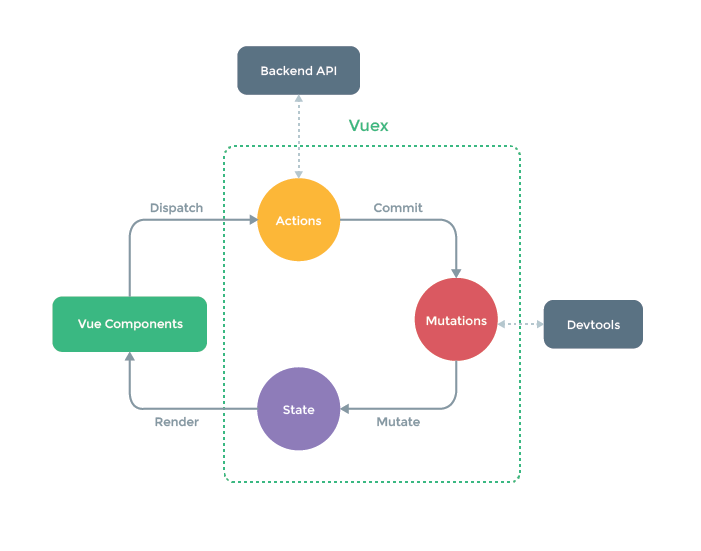
\includegraphics[width=\textwidth]{images/vuex.png}
	\caption{Diagram znázorňující životní cyklus dat v knihovně Vuex}
	%TODO: Popsat v obrázku nebo v textu?
	%[https://vuex.vuejs.org/ 24.4.]
	\label{vuex-dataflow}
\end{figure}

\blindtext

\subsubsection*{BootstrapVue}

\section{Elasticsearch}
%[https://books.google.cz/books?hl=cs&lr=&id=d19aBgAAQBAJ&oi=fnd&pg=PR3&dq=elasticsearch&ots=NzhZuNHtgB&sig=zWUdusVrNdR1BvbOtj8YZ43G-oM&redir_esc=y#v=onepage&q=elasticsearch&f=false 29.4.]
Elasticsearch je volně šiřitelný vyhledávač umožňující distribuované vyhledávání a analýzu v reálném čase. Umožňuje rychle pracovat s rozsáhlými daty (anglicky \emph{big data}) a provádět nad nimi plnotextové vyhledávání, strukturované vyhledávání a nebo zmiňovanou analýzu.

Tento vyhledávač je hojně využíván jak menšími projekty, tak i světoznámými organizacemi. Za zmínku stojí například internetová encyklopedie Wikipedia\footnote{Wikipedia: \url{https://www.wikipedia.org/}}, britský deník The~Guardian\footnote{The Guardian: \url{https://www.theguardian.com/international}}, komunitní stránka pro výměnu rad programátorů StackOverflow\footnote{StackOverflow: \url{https://stackoverflow.com/}} nebo populární webová služba pro verzovací nástroj Git a to GitHub\footnote{GitHub: \url{https://github.com/}}.

Elasticsearch je postavený na knihovně Apache Lucene\footnote{Apache Lucene: \url{https://lucene.apache.org/}}, využívá především její funkce plnotextového vyhledávání, ale oproti této knihovně samotné Elasticsearch nabízí o mnoho přívětivější způsob používání, především pro začínající uživatele. 

Jedná se o bezschémovou databázi, oproti relačním databázím nenabízí propojovací dotazy, a proto je nutné ukládaná data denormalizovat. Díky tomu jsou ale data a jejich metadata v těsné blízkosti a tím je docíleno rychlé fulltextové vyhledávání. %[https://qbox.io/blog/what-is-elasticsearch 20.4.]

\subsection{Základní struktura}
Základní struktura databáze Elasticsearch se na první pohled od tradičních relačních databázi velmi neliší, ke spoustě pojmů se dá najít ekvivalent.

\subsubsection*{Uzel a shluk}
Pod pojmem uzel (anglicky \emph{node}) se skrývá server, ve kterém jsou uložena data. Uzel v rámci databáze může být jeden nebo jich může být i více a každý bude obsahovat pouze určitou část dat. Tyto uzly jsou seskupeny do shluku (anglicky cluster).

\subsubsection*{Dokument}\label{section:dokument}
Dokument je základní jednotka dat, které může být zaindexována. Obsah dokumentu je zapsán ve formátu JSON. V relační databázi lze dokument přirovnat k řádku tabulky.

\subsubsection*{Index}\label{section:index}
Skupina dokumentů s podobnou strukturou se nazývá index. Ekvivalentem v relačních databázích by v tomto případě byla tabulka.

\subsubsection*{Střepy}
Elasticsearch nabízí možnost index rozdělit na střepy (anglicky \emph{shards}), které mohou být uloženy v různých uzlech. Tuto možnost je vhodné využít především při práci s indexy s velkým obsahem dat. Díky rozdělení docílíme distribuování zátěže a lze využít paralelní zpracování, tudíž bude zpracování dotazu odbaveno výrazně rychleji. 
Přístup k takto rozděleným indexům se nijak nemění a pro uživatele je tento proces naprosto transparentní.

\subsubsection*{Repliky}
Obdobně lze využít i repliky. Zde se ovšem data indexu nerozdělují, ale naopak duplikují. Díky uložení těchto replik mezi více uzly může systém být robustnější a dokáže fungovat i v případě selhání části shluku. I v tomto případě je umožněno vyhledávat paralelně. 

\subsection{Dotazy}
Pro komunikaci s touto databází se využívá Query DSL - dotazy aplikačního rozhraní REST ve formátu JSON.

Obsah dotazu může vypadat například následovně
\begin{verbatim}
{
    "query": {
        "match": {
            "address": "todo"
        }
    }
}
\end{verbatim} %TODO: Jiny priklad

Na tento dotaz můžeme od serveru dostat odpověď s obsahem

\blindtext

\subsubsection*{Kontext}
Dotazy v Elasticsearch se rozlišují na dva základní typy - kontext dotazu (\emph{query}) a kontext filtru.
První z nich se dá lidsky přeložit do otázky \uv{Jak moc dokument splňuje dotaz?}. V tomto případě se u každého výsledku počítá skóre relevance, podle kterého jsou ve výsledné odpovědi dokumenty sestupně řazeny.

\subsection{Metadata}
\blindtext

\subsection{Fasetové vyhledávání}
S velkým množstvím dat přichází potřeba obsah podle určitých kriterií zúžit. K tomutu účelu slouží filtry a fasetové vyhledávání (někdy také označována jako fastová navigace - anglicky \emph{faceted search} nebo \emph{faceted navigation}). Využití faset je ale pokročilejší než použít filtry, protože fasetová navigace umožňuje využít hned několik filtrů najednou. %[https://www.nngroup.com/articles/filters-vs-facets/ 21.4.]

V Elasticsearch je možné tuto navigaci vytvořit pomocí tzv. kyblíkových agreagací (angl. \emph{bucket aggregations}).
Jednoduše řečeno, se pro dokumenty vytvoří kyblíky, kde každý z kyblíku odpovídá určitému kriteriu. Pokud dokument toto kriterium splňuje, je do kyblíku vložen.
%[https://www.elastic.co/guide/en/elasticsearch/reference/current/search-aggregations-bucket.html 21.4.]

\subsection{Plnotextové vyhledávání}
%[https://books.google.cz/books?hl=cs&lr=&id=d19aBgAAQBAJ&oi=fnd&pg=PR3&dq=elasticsearch&ots=NzhZuNHtgB&sig=zWUdusVrNdR1BvbOtj8YZ43G-oM&redir_esc=y#v=snippet&q=full&f=false 29.4.]
Uložená data se dělí na dva typy - přesné hodnoty a plnotextové hodnoty (anglicky \emph{full-text}). Přesné hodnoty jsou určeny pro data, jako například identifikátor uživatele. Pokud totiž vyhledáváme uživatele s identifikátorem 42, jako výsledek neočekáváme uživatele, který má identifikátor 420, ale očekáváme výsledek, který bude přesně splňovat hledanou položku.
Pokud ale člověk pracuje s textovými položkami, nemusí nutně hledat stoprocentní shodu. Lidský jazyk je velice rozmanitý a umožňuje slova časovat, skloňovat, či vyjádřit jednu věc vícero synonyma. %todo sklonuju spravne?
V těchto případech hledání totožných hodnot selhává, i když má text z pohledu člověka stejný nebo podobný význam. Pro tento typ hledání slouží právě plnotextové hledání. Můžeme se s ním setkat například při hledání článku v internetovém magazínu.
Elasticsearch pro takové hledání musí text nejprve analyzovat a vytvořit pro něj obrácené indexy.

\subsubsection*{Obrácený index}
Obrácený index (anglicky \emph{inverted index}) je struktura obsahující seznam všech unikátních slov vyskytujících se v uložených dokumentech. Pro každé z těchto slov uchovává informaci, ve kterých dokumentech se vyskytovalo. Díky tomu je možné v textových položkách rychle provádět plnotextové hledání.

Příkladem mohou být dva dokumenty, kde každý obsahuje právě jednu z následujících vět.
\begin{itemize}
    \item 
    \item 
\end{itemize}
Zpracování těchto dokumentů tedy může vzniknout následující obrácený index
%TODO table
Takovýto index by byl ale v praxi nepoužitelný. Text nestačí pouze strojově rozdělit do tokenů, ale musí proběhnout celá analýza textu.

\subsubsection*{Analýza}
Analýza představuje proces, kdy se kus textu rozdělí do jednotlivých tokenů a následně se tyto tokeny upraví do podoby vhodné pro použití plnotextového vyhledávání. Tento proces obstarává analyzér, který se skládá ze tří části:
\begin{itemize}
    \item \emph{Filtry znaků} upraví zpracovávaný řetězec ještě před samotným rozdělením do tokenů. Jeho úkolem může například být odstranění HTML značek z textu.
    \item \emph{Tokenizér} z textu sestaví jednotlivé tokeny. Tokeny ve většině případů představují jednotlivá slova, ale nemusí tomu tak vždy být. 
    \item \emph{Filtry tokenů} na konec projde všechny vytvořené tokeny, může některé odstranit, přidat a nebo jen upravit. 
\end{itemize}
Filtrů může být v jednom analyzéru použitá celá řada a to jak filtrů znaků, tak i filtrů tokenů. Tokenizér je ale v rámci analyzéru vždy použit jen jeden jediný.

Elasticsearch již ve svém základu nabízí škálu různých analyzéru. Tyto analyzéry jsou různé složitosti, mezi ty nejjednodušší patří analyzér bílých znaků, který text rozdělí striktně podle mezer, tudíž je i tečka na konci věty vnímána jako část slova. Nejčastěji se ale člověk může setkat s jazykovým analyzérem, který je uzpůsoben lidské řeči. Elasticsearch takový analyzér nabízí pro mnoho jazyků mezi které patří i jazyk český.

\subsubsection*{Filtry tokenů}
%https://www.ludekvesely.cz/serial-elasticsearch-4-fulltextove-vyhledavani-v-cestine/ 2.4.

Velmi častou filtrací bývá změna velkých písmen na malé, díky tomu nejsou slova na začátku věty vnímána jako jiná slova, než ty v jiné části věty. Pro český jazyk je také typické odstranění diakritiky.

Součástí analyzátorů bývá často odstranění tokenů, které obsahují nepodstatná slova. Jedná se především o spojky a předložky. Taková slova se v plnotextovém vyhledávání označují jako \emph{stop slova} (anglicky \emph{stop words}). Tento seznam je vždy specifický pro konkrétní jazyk textu, použít výchozí anglická stop slova nad česky psaným textem by ztrácelo význam.

Další nedílnou součástí pokročilejších analyzátorů je \emph{stematizace}, aneb převod slov do jejich základního tvaru. Pro tuto operaci lze využit dva způsoby a to algoritmus nebo slovník. Každý z těchto způsobů má své pro a proti.
Využitím algoritmické stematizace sice analyzátor nemusí znát všechna slova v daném jazyce, protože slova převádí do základního tvaru pouze na základě sady pravidel, ale zase dochází k určité nepřesnosti. Elasticsearch v případě využití české algoritmické stematizace ze slov odstraňuje všechny přípony.
Druhým způsobem, který lze využít je stematizace na základě slovníku. Díky tomu jsou převedené tvary přesnější než ty získané algoritmem, ale hlavním předpokladem je využití vhodného slovníku s dostatečnou zásobou slov.
%TODO priklad

\subsection{Podobnostní hledání}
\blindtext[2]

\subsection{Knihovny}
\blindtext[2]